\section{GAN para Colorización}

Tras evaluar modelos deterministas como autoencoders y VAEs, ahora vamos a explorar un enfoque basado en redes GAN para la colorización. Las GAN son especialmente adecuadas para esta tarea porque incorporan un discriminador que empuja al generador a producir colores más realistas y coherentes, incluso en zonas donde la elección del color es más ambigua. Esto suele traducirse en imágenes más saturadas, con transiciones suaves y menos aspecto borroso que en los métodos puramente reconstrucción.

Nuestro modelo sigue la filosofía de \textit{pix2pix}\cite{isola2017pix2pix}, formulando la colorización como un problema de \textit{image-to-image translation}: dado el canal L de luminancia de una imagen en espacio Lab, el objetivo es predecir los canales a y b que contienen la información cromática.

\subsection{Arquitectura del Generador U-Net}

Para el generador empleamos una U-Net \cite{ronneberger2015unet}, debido a su capacidad para preservar la información espacial de la imagen gracias a sus skip conexions entre encoder y decoder. En colorización esto es crucial porque aunque el color pueda variar, los bordes, contornos y texturas deben mantenerse.

\begin{figure}[H]
\centering
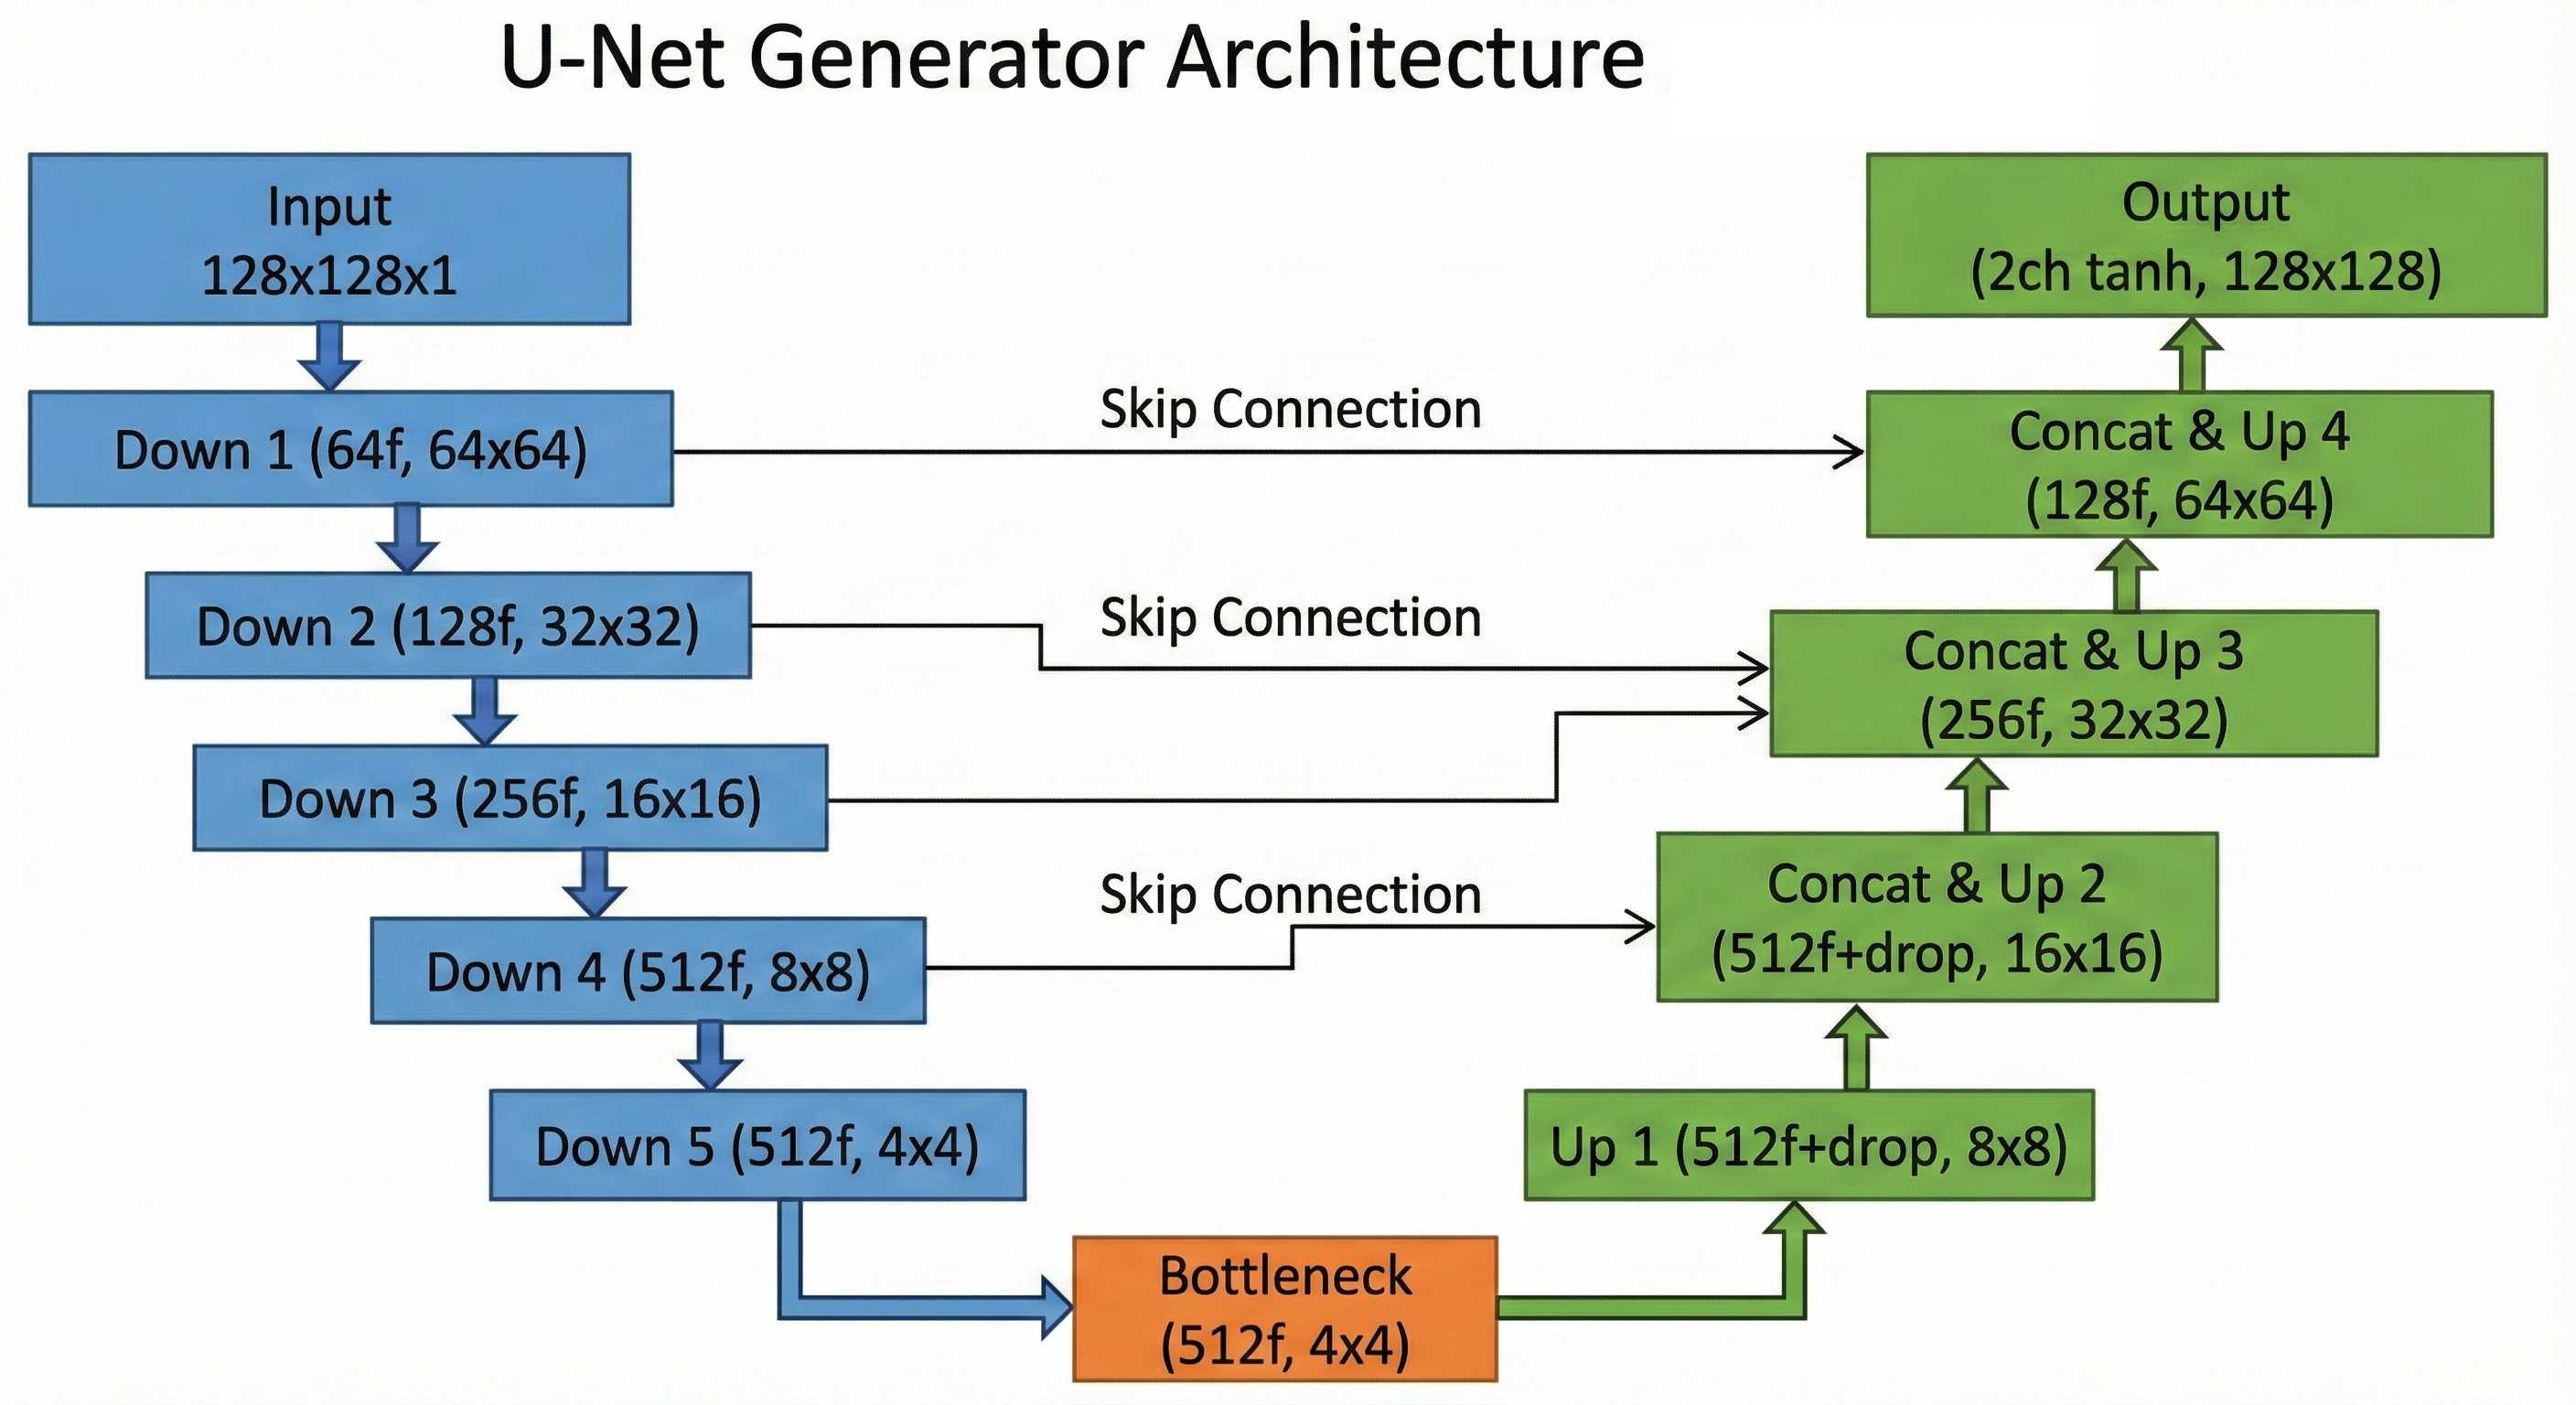
\includegraphics[width=0.75\linewidth]{images/unet_diagram.png}
\caption{Diagrama de la arquitectura U-Net}
\label{fig:unet_generator}
\end{figure}

El generador recibe como entrada un tensor de dimensiones $(128\times128\times1)$ con la imagen en escala de grises. Su estructura se organiza en dos partes:

\begin{itemize}
    \item \textbf{Bloques de downsampling}: cinco niveles de convoluciones 4×4 con \textit{stride} 2, que van reduciendo la resolución mientras aumentan los filtros (64, 128, 256, 512, 512). Todas las capas salvo la primera incluyen BatchNorm. Se emplea activación LeakyReLU.
    
    \item \textbf{Bloques de upsampling}: cuatro capas transpuestas de convolución para recuperar la resolución. Los dos primeros bloques incorporan \textit{dropout} (0.5), lo que introduce variabilidad para evitar que el generador memorice patrones del entrenamiento y se dé sobreajuste.

    \item \textbf{Skip conexions}: cada bloque de upsampling concatena su salida con el mapa correspondiente del encoder. Esto permite reconstruir detalles finos, evitando que se pierda información por el downsampling.

    \item \textbf{Salida}: una convolución transpuesta adicional produce una imagen $(128\times128\times2)$ con activación \textit{tanh}, que corresponde a los canales a y b normalizados [-1,1].
\end{itemize}

En conjunto, la U-Net hace que las colorizaciones sean más nítidas, evitando que la red rellene grandes áreas con colores uniformes o poco detallados.

\subsection{Arquitectura del Discriminador PatchGAN}

Para el discriminador vamos a utilizar una variante de \textit{PatchGAN} al igual que se hace en \textit{pix2pix}\cite{isola2017pix2pix}, que en lugar de emitir una única predicción global de la imagen, produce un mapa de activación donde cada celda evalúa si el parche correspondiente parece real o generado. 

Una particularidad de nuestro modelo es que el discriminador, además del mapa de activación de real/falso, devuelve características intermedias de varias capas. Estas representaciones se emplean para calcular una \textit{Feature Matching Loss}, que hace que el entrenamiento sea más estable y ayuda al generador hacia distribuciones más coherentes.
Esta técnica fue introducida por Salimans et al.~\cite{salimans2016improved} y ayuda mejorar la calidad perceptual de la GAN, obligando al generador a reproducir las estadísticas internas del discriminador en vez de centrarse únicamente en engañarlo, esto nos va a ayudar a que los colores sean más vivos y no se dé mode-collapse.

Su estructura es la siguiente:

\begin{itemize}
    \item Recibe la imagen de entrada L y la imagen objetivo o generada ab, formando un tensor $(128\times128\times3)$.
    \item Aplica tres bloques de convolución 4×4 con \textit{stride} 2, aumentando progresivamente el número de filtros (64, 128, 256).
    \item Añade dos convoluciones adicionales sin reducir la resolución.
    \item Produce un mapa final $(14\times14\times1)$ con las predicciones por parche.
    \item Devuelve además las activaciones de varias capas internas para la feature loss.
\end{itemize}

Esto nos permite capturar errores que se dan forma local en ciertas partes de la imagen, que una discriminador global podría pasar por alto.

\subsection{Funciones de pérdida}

La pérdida total del generador combina tres términos:

\begin{itemize}
    \item \textbf{Pérdida adversaria} (\( \mathcal{L}_{GAN} \)): empuja al generador a producir colores que el discriminador no pueda distinguir de los reales.

    \item \textbf{Pérdida L1} (\( \mathcal{L}_{L1} \)): calcula el error absoluto medio entre los canales de color reales y generados. Favorece soluciones estables y evita saltos o colores irreales.

    \item \textbf{Feature Matching Loss} (\( \mathcal{L}_{FM} \)): mide la diferencia entre las activaciones intermedias que el discriminador produce para imágenes reales y generadas. Esto actúa como una regularización y reduce el mode-collapse.
\end{itemize}

El coste total del generador es:

\[
\mathcal{L}_G = \mathcal{L}_{GAN} + \lambda \mathcal{L}_{L1} + \lambda \mathcal{L}_{FM},
\]

empleando \( \lambda = 10 \), un valor que balancea adecuadamente la reconstrucción y la calidad perceptual.

El discriminador minimiza:

\[
\mathcal{L}_D = \mathcal{L}_{real} + \mathcal{L}_{fake}.
\]

Ambas pérdidas se implementan mediante \textit{binary cross-entropy} con logits.

\subsection{Entrenamiento}

Entrenamos tanto el generador como el discriminador con Adam, usando una tasa de aprendizaje de \(2 \cdot 10^{-4}\) y \(\beta_1 = 0.5\), siguiendo las recomendaciones clásicas en GANs.

Durante cada iteración del entrenamiento:

\begin{enumerate}
    \item El generador predice los canales de color a partir del canal L.
    \item El discriminador evalúa tanto la pareja real (L + ab) como la generada (L + \(\hat{ab}\)).
    \item Se extraen activaciones intermedias del discriminador para calcular \(\mathcal{L}_{FM}\).
    \item Se calculan las pérdidas y se actualizan ambos modelos.
\end{enumerate}

Entrenamos el modelo durante 50 epochs utilizando el dataset STL al igual que en los modelos anteriores pero tomando un subset de 20.000 imágenes unlabeled para el entrenamiento, 1.000 para validación y 8.000 para test. Todas las imágenes se redimensionaron a \(128\times128\) y se transformaron al espacio Lab usando \textit{skimage}.

\subsection{Resultados}

Para evaluar el rendimiento de la GAN clásica utilizamos las tres métricas anteriores:
SSIM, que mide la coherencia estructural; PSNR, que cuantifica la fidelidad de reconstrucción,
y LPIPS, que evalúa la similitud perceptual.

\begin{table}[H]
\centering
\caption{Métricas de evaluación de la GAN}
\label{tab:gan_metrics}
\vspace{0.2cm}
\begin{tabular}{lc}
\hline
\textbf{Métrica} & \textbf{GAN} \\ \hline
SSIM  & 0.9097 \\ 
PSNR  & 23.6826 \\ 
LPIPS & 0.1628 \\ \hline
\end{tabular}
\end{table}

Las métricas reflejan que el modelo es capaz de preservar adecuadamente la estructura global de la imagen 
(SSIM = 0.91), aunque todavía existe un error de reconstrucción apreciable (PSNR = 23.7),
como es de esperar por la dificultad inherente de la colorización. El valor de LPIPS ($0.1628$) indica que,
a nivel perceptual, las predicciones son razonablemente cercanas a las imágenes reales,
pero aún presentan errores en la coloración de zonas más ambiguas.

En la Figura~\ref{fig:gan_results} podemos ver algunos de los ejemplos del conjunto de test,
comparando las imágenes originales en escala de grises con las generadas y la original a color.

\begin{figure}[H]
\centering
\begin{minipage}{0.48\linewidth}
    \centering
    \includegraphics[width=\linewidth, keepaspectratio]{images/gan-2.png}
\end{minipage}\hfill
\begin{minipage}{0.48\linewidth}
    \centering
    \includegraphics[width=\linewidth, keepaspectratio]{images/gan-3.png}
\end{minipage}

\caption{Resultados cualitativos de la GAN.}
\label{fig:gan_results}
\end{figure}

Como podemos ver con las GAN, las imágenes resultantes tienen colores más saturados y con mejor continuidad que con los autoencoders y VAEs, especialmente si son objetos con bordes bien definidos o texturas sencillas.

Aún asi el modelo sigue mostrando ciertas ambigüedades en regiones donde el color real no está bien determinado, lo cual es esperable en colorización.

\section{GAN Guiada por Segmentación}

Tras comprobar que la GAN clásica si que colorea las imágenes decentemente, para solucionar algunas de las ambigüedades que ya hemos mencionado, probamos a mejorar este enfoque incorporandole información semántica mediante segmentación. La motivación principal es que muchos errores cromáticos pasan por la falta de contexto, es decir, la GAN no sabe si una región gris corresponde a cielo, agua, vegetación o a un objeto en concreto.  

Para resolver esto hemos complementado nuestra GAN con segmentación utilizando SegFormer, que nos proporciona una máscara semántica de la imagen pixel por pixel. Este mapa nos sirve como entrada extra para el generador, y le ayuda a colorear de forma más coherente con los diferente elementos de la escena.

\subsection{Obtención de Máscaras Semánticas con SegFormer}

Para obtener las máscaras hemos utilizado SegFormer-B0 \cite{xie2021segformer}, un modelo \textit{transformer-based} preentrenado sobre ADE20K, que destaca por su buen equilibrio entre precisión y velocidad. Antes de escoger SegFormer como modelo de segmentación, probamos a utilizar \textit{Segment Anything Model} (SAM) \cite{kirillov2023sam}, dado que es uno de los métodos más recientes y precisos. Sin embargo, en la práctica SAM resultó muy costoso computacionalmente para los recursos que teniamos. 
Por estas razones descartamos SAM y optamos por SegFormer-B0 que es un modelo mucho más eficiente computacionalmente.
Para cada imagen en RGB del dataset generamos un mapa de logits de dimensión $(150,H,W)$, que corresponde a las clases originales de ADE20K. Este mapa se interpola a la resolución original y se obtiene la clase más probable en cada píxel:

\[
\text{mask}_{150}(x,y) = \arg\max_c \; \text{logits}[c,x,y].
\]

Dado que 150 clases son demasiado detalladas para nuestro problema y generan ruido innecesario, las reducimos a un conjunto de 9 clases semánticas mas relevantes en nuestro dataset:

\begin{itemize}
    \item cielo,  
    \item vegetación,  
    \item agua,  
    \item animales,  
    \item persona/cuerpo,  
    \item vehículos,  
    \item estructuras/edificios,  
    \item objetos pequeños,  
    \item fondo.
\end{itemize}

Después convertimos estas etiquetas a one-hot:

\[
S \in \mathbb{R}^{9 \times 128 \times 128}.
\]

Estas máscaras una vez generadas las almacenamos como archivos \texttt{.npy}, para entrenar con ellas posteriormente.

\subsection{Integración de la Máscara en la GAN}

El generador ahora recibe como entrada no solo el canal L, sino también los 9 canales de la segmentación:

\[
G([L, S]) \rightarrow \hat{ab}.
\]

Esto expande la entrada de la U-Net de 1 a 10 canales, haciendo que desde el primer nivel del encoder el modelo pueda ver el contenido semántico de la imagen.  

El discriminador se mantiene con la misma estructura PatchGAN anterior, evaluando el par \((L, \hat{ab})\), ya que su función es juzgar el realismo del color, no la semántica.

\subsection{Función de Pérdida}

La GAN guiada por segmentación mantiene exactamente la misma configuración de pérdidas que la GAN clásica, 
ya que el objetivo del modelo no cambia: generar unos canales $ab$ cromáticamente coherentes 
con la imagen real. La introducción de la máscara semántica afecta únicamente a la entrada del generador, pero no altera el resto de la arquitectura adversarial.

Así, la pérdida total del generador combina tres términos:

\[
\mathcal{L}_G = \mathcal{L}_{GAN} + \lambda_{1}\mathcal{L}_{L1} + \lambda_{2}\mathcal{L}_{FM},
\]

donde:

\begin{itemize}
    \item \textbf{$\mathcal{L}_{GAN}$: pérdida adversaria}. Incentiva que el generador produzca imágenes 
    que el discriminador clasifique como reales.

    \item \textbf{$\mathcal{L}_{L1}$: pérdida de reconstrucción}. Mide la diferencia absoluta promedio entre 
    los canales reales y generados. Su papel es estabilizar el aprendizaje y evitar desviaciones cromáticas excesivas.

    \item \textbf{$\mathcal{L}_{FM}$: Feature Matching Loss}. Calcula la distancia entre las activaciones 
    internas del discriminador para imágenes reales y generadas. Actúa como regularizador y ayuda a estabilizar 
    el entrenamiento adversarial.
\end{itemize}

Siguiendo la misma configuración que en la GAN sin segmentación, empleamos $\lambda_1 = 10$ y $\lambda_2 = 10$, 
que mantienen un equilibrio entre fidelidad cromática y calidad perceptual.

El discriminador utiliza la misma pérdida adversarial que en el modelo clásico:

\[
\mathcal{L}_D = \mathcal{L}_{real} + \mathcal{L}_{fake},
\]

evaluando únicamente si el par $(L, \hat{ab})$ es realista, ya que su función no requiere información semántica.

\subsection{Entrenamiento}

Mantenemos la misma configuración que en la GAN básica:

\begin{itemize}
    \item Optimizador Adam (\texttt{lr = $2\cdot 10^{-4}$}, \(\beta_1 = 0.5\)),  
    \item Imagen de entrada: canal L normalizado en \([-1,1]\),  
    \item Máscara semántica: mapa one-hot de 9 canales,  
    \item Resolución final: \(128 \times 128\),  
    \item Batch size: 32,  
    \item Epochs: 50.
\end{itemize}

\subsection{Resultados y Métricas}

Al evaluar el rendimiento del modelo guiado con segmentación, vemos que las métricas cuantitativas 
son muy similares a las obtenidas por la GAN clásica. Esto es esperable, dado que las métricas como SSIM 
y PSNR no capturan directamente la coherencia semántica del color, sino aspectos puramente estructurales 
o de reconstrucción.

\begin{table}[H]
\centering
\caption{Métricas de evaluación de la GAN guiada por segmentación}
\label{tab:seg_gan_metrics}
\vspace{0.2cm}
\begin{tabular}{lc}
\hline
\textbf{Métrica} & \textbf{GAN + Segmentación} \\ \hline
SSIM  & 0.9073 \\ 
PSNR  & 23.3946 \\ 
LPIPS & 0.1660 \\ \hline
\end{tabular}
\end{table}

\begin{figure}[H]
    \centering
    \begin{minipage}{0.48\linewidth}
        \centering
        \includegraphics[width=\linewidth, keepaspectratio]{images/seg_gan.png}
    \end{minipage}\hfill
    \begin{minipage}{0.48\linewidth}
        \centering
        \includegraphics[width=\linewidth, keepaspectratio]{images/seg_gan-2.png}
    \end{minipage}
    
    \caption{Resultados cualitativos del modelo con segmentación.}
    \label{fig:seg_gan_results}
    \end{figure}

A nivel cualitativo, destacamos los siguientes efectos positivos derivados de la segmentación:

\begin{itemize}
    \item \textbf{Mayor coherencia cromática en clases} como en el cielo, agua o vegetación.
    
    \item \textbf{Reducción del \textit{color bleeding}} en contornos de objetos, especialmente 
    en personas, animales o vehículos. La máscara impide que el color se extienda a regiones 
    incorrectas.
\end{itemize}

Aunque las métricas muestran un rendimiento similar al de la GAN sin segmentación, el análisis visual 
revela mejoras en la coherencia del color. En los ejemplos del conjunto de test, se aprecia cómo la segmentación guía al generador 
a producir colorizaciones más consistentes con el contenido semántico de la imagen.

No obstante, también observamos que cuando la segmentación de SegFormer es incorrecta, 
el generador puede reproducir errores similares a los de la GAN clásica o incluso colorear regiones de un color que no les corresponde, por ejemplo, colorear la tierra como si fuera césped. Aun así, el modelo se 
mantiene estable y no empeora significativamente, lo que indica que la arquitectura no se degrada 
incluso teniendo ruido semántico.

En conjunto, aunque las métricas cuantitativas no mejoran de forma sustancial, la calidad 
perceptual sí lo hace ligeramente, especialmente en escenas donde la semántica es determinante para la elección 
del color. Cabe destacar que una de las posibles razones por las que la incorporación de segmentación no produce una mejora significativa es la baja resolución de las imágenes del dataset. 
Al trabajar con imágenes de $128 \times 128$ píxeles, las máscaras generadas tienden a ser poco precisas en regiones pequeñas, lo que hace que el generador no reciba información semántica relevante. En estos casos, la segmentación no introduce un contexto semántico suficientemente rico como para influir de manera notable en el proceso de colorización.
